\test{Structure Integration}\label{test:struct_integ}
\begin{description}
\item[Background] The primary purpose of this test is to test that
integrating the structural origin yields very similar results compared
to integrating the composite body center of mass.

\item[Test description]
This test uses a near-carbon copy of \verb+$JEOD_HOME/verif/SIM_dyncomp+, with
a StructureIntegratedDynBody replacing the DynBody used in that
simulation. \verb+SIM_dyncomp+ has been cross-validated with a number of
external simulations. Cross-checking the near-carbon copy demonstrates that
the structure-integrated dynamic body code provides valid results.

\item[Test directory]
{\tt models/dynamics/dyn\_body/verif/SIM\_dyncomp\_structure} \\
The simulation \Sdefine file replaces the DynBody used in
\verb+SIM_dyncomp+ with a StructureIntegratedDynBody.
The \verb+S_overrides.mk+ file generates the \verb+SET_test+ run directories
by copying the corresponding python input files from the corresponding
\verb+SIM_dyncomp+ run directories. The The \verb+S_overrides.mk+ file also
makes the \verb+Modified_data+ and \verb+Log_data+ directories be symbolic
links to the corresponding directories in \verb+SIM_dyncomp+. These acts ensure
that \verb+SIM_dyncomp_structure+ simulation runs start under the same
initial conditions as do the corresponding \verb+SIM_dyncomp+ runs.

\item[Success criteria] Corresponding runs of \verb+SIM_dyncomp+ and
\verb+SIM_dyncomp_structure+ should agree to high degree of precision
throughout the eight hour span of the \verb+SIM_dyncomp+ runs.
To test this, position discrepencies must be small, on the order of
millimeters at most.

\item[Test results] The magnitudes of the position discrepancies
between \verb+SIM_dyncomp+ and the structure-integrated replacement
for the the four most sensitive \verb+IM_dyncomp+ runs are depicted in
figure~\ref{fig:SIM_dyncomp_RUN_10_discrepancies}. The largest discrepancies
are less than 100 micrometers, even on the one test case that shows the
greatest deviation. These small errors are purely numerical.

The test passes.

\item[Applicable requirements]
This test demonstrates the partial or complete satisfaction of the
following requirements:
\begin{itemize}
\item \ref{reqt:eom}. Forces and torques are properly accumulated and
propagated. Accelerations are properly calculated from forces and torques.
\item \ref{reqt:state_integ_prop}. The equations of motion are properly
integrated.
\end{itemize}

\end{description}

\begin{figure}[hbtp]
\centering
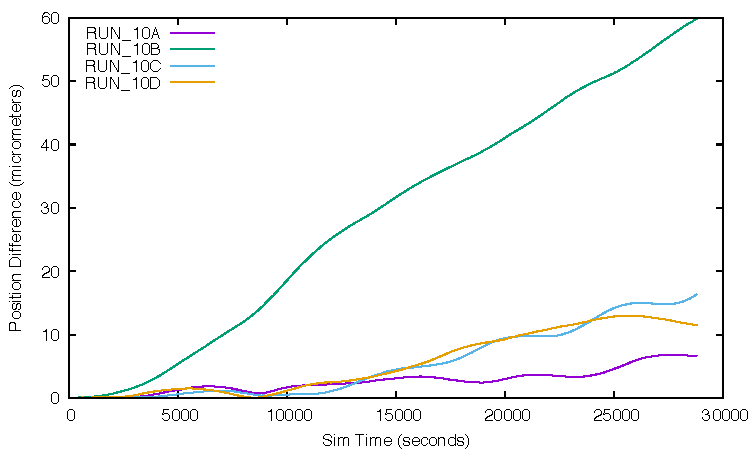
\includegraphics{SIM_dyncomp_compare.pdf}
\caption{Structural origin vs center of mass integration position discrepancies}
\label{fig:SIM_dyncomp_RUN_10_discrepancies}
\end{figure}
